\documentclass{article}
\usepackage{graphicx}
\usepackage[margin=1.5cm]{geometry}
\usepackage{amsmath}
\usepackage{hyperref}
\hypersetup{
    colorlinks=true,
    linkcolor=blue,
    filecolor=magenta,      
    urlcolor=cyan,
    pdftitle={Overleaf Example},
    pdfpagemode=FullScreen,
}

\begin{document}
\twocolumn

\title{Quiz 3: Digital Signal Processing}
\author{Prof. Jordan C. Hanson}

\maketitle
\small

\section{Spectrograms, DFTs, and Chirped Signals}

\begin{enumerate}
\item According to the \textbf{Doppler effect}, the frequency of electromagnetic waves reflecting from a moving target will shift in proportion to the velocity of the target.  Let $f_t$ represent the transmitted frequency, $f_r$ represent the reflected frequency, and $f_d = f_r - f_t$.  To first order in $v/c$, 
\begin{equation}
f_d \approx 2 v \frac{f_t}{c}
\end{equation}
(a) Suppose the relative velocity $v$ between our craft and the enemy fighter is $v \approx 300$ m s$^{-1}$, and our radar operates at 1 GHz.  What is the Doppler shift, $f_d$? (b) Given that our receiver has to resolve the difference between $f_t = 1$ GHz and $f_t+f_d$, for how long do we have to record the reflected waveform? That is, how do we achieve the required frequency resolution? (c) If we sample at 2 GHz, how many samples would be in the waveform?  Is this practical?
\item Consider the radar spectrogram illustrated in Fig. \ref{fig:1}.  Our craft produces a chirped pulsed radar transmission that echoes from the enemy craft from a distance $R$.  Our transmitted signal is a linear chirp with a slope $k$, usually in MHz/$\mu$s.  (a) Let $c$ be the speed of light, $\Delta f$ and $\Delta t$ be the changes in frequency and time ($k=\Delta f/\Delta t$), and $R$ be the \textit{range} to the other craft.  Show that
\begin{equation}
R = \frac{c}{2k}\Delta f \label{eq:1}
\end{equation}
(b) Equation \ref{eq:1} implies that the difference between the most powerful frequencies at a fixed time, $\Delta f$, can be translated into a target \textit{range.}  Suppose our system detects $\Delta f = 25$ MHz, with $k = 1$ MHz/$\mu$s, and $c = 300$ m MHz.  What is $R$, in km?
\item \textbf{Download the \textbf{\href{https://cms.whittier.edu/mod/resource/view.php?id=683184}{Radar Data for Quiz 3}}} from our course Moodle page.  The file is a $N \times 2$ data set with units of seconds and volts.  Write an \verb+octave+ script to compute the spectrogram of the data, and share the graph.
\item Once the spectrogram is graphed, answer the following questions, using any and all relevant DSP techniques:
\begin{itemize}
\item Select a time at which the transmission and echo signals overlap.  One way to measure $\Delta f$ is the \verb+findpeaks()+ in the \verb+octave+ package \verb+signal+. Calculate $\Delta f$ in MHz.
\item What is the range to the enemy craft, in km?
\item \textit{Wait ... how many enemy craft are there?} What is the distance to the \textbf{second} aircraft, in km?
\end{itemize}
\end{enumerate}

\vspace{3cm}

\section{Linear Image Processing}

\begin{enumerate}
\item \textbf{Download the \textbf{\href{https://cms.whittier.edu/mod/resource/view.php?id=683189}{Image Data for Quiz 3}}} from our course Moodle page.  The file is a $N \times M$ image with greyscale pixels.
\item Create an appropriate $3 \times 3$ filter kernel to filter the image.  Filter the image to reduce noise and enhance the edges.
\item What is the number written below and behind the cockpit?
\item \textbf{Bonus:} What type of aircraft is this?
\end{enumerate}

\begin{figure}
\centering
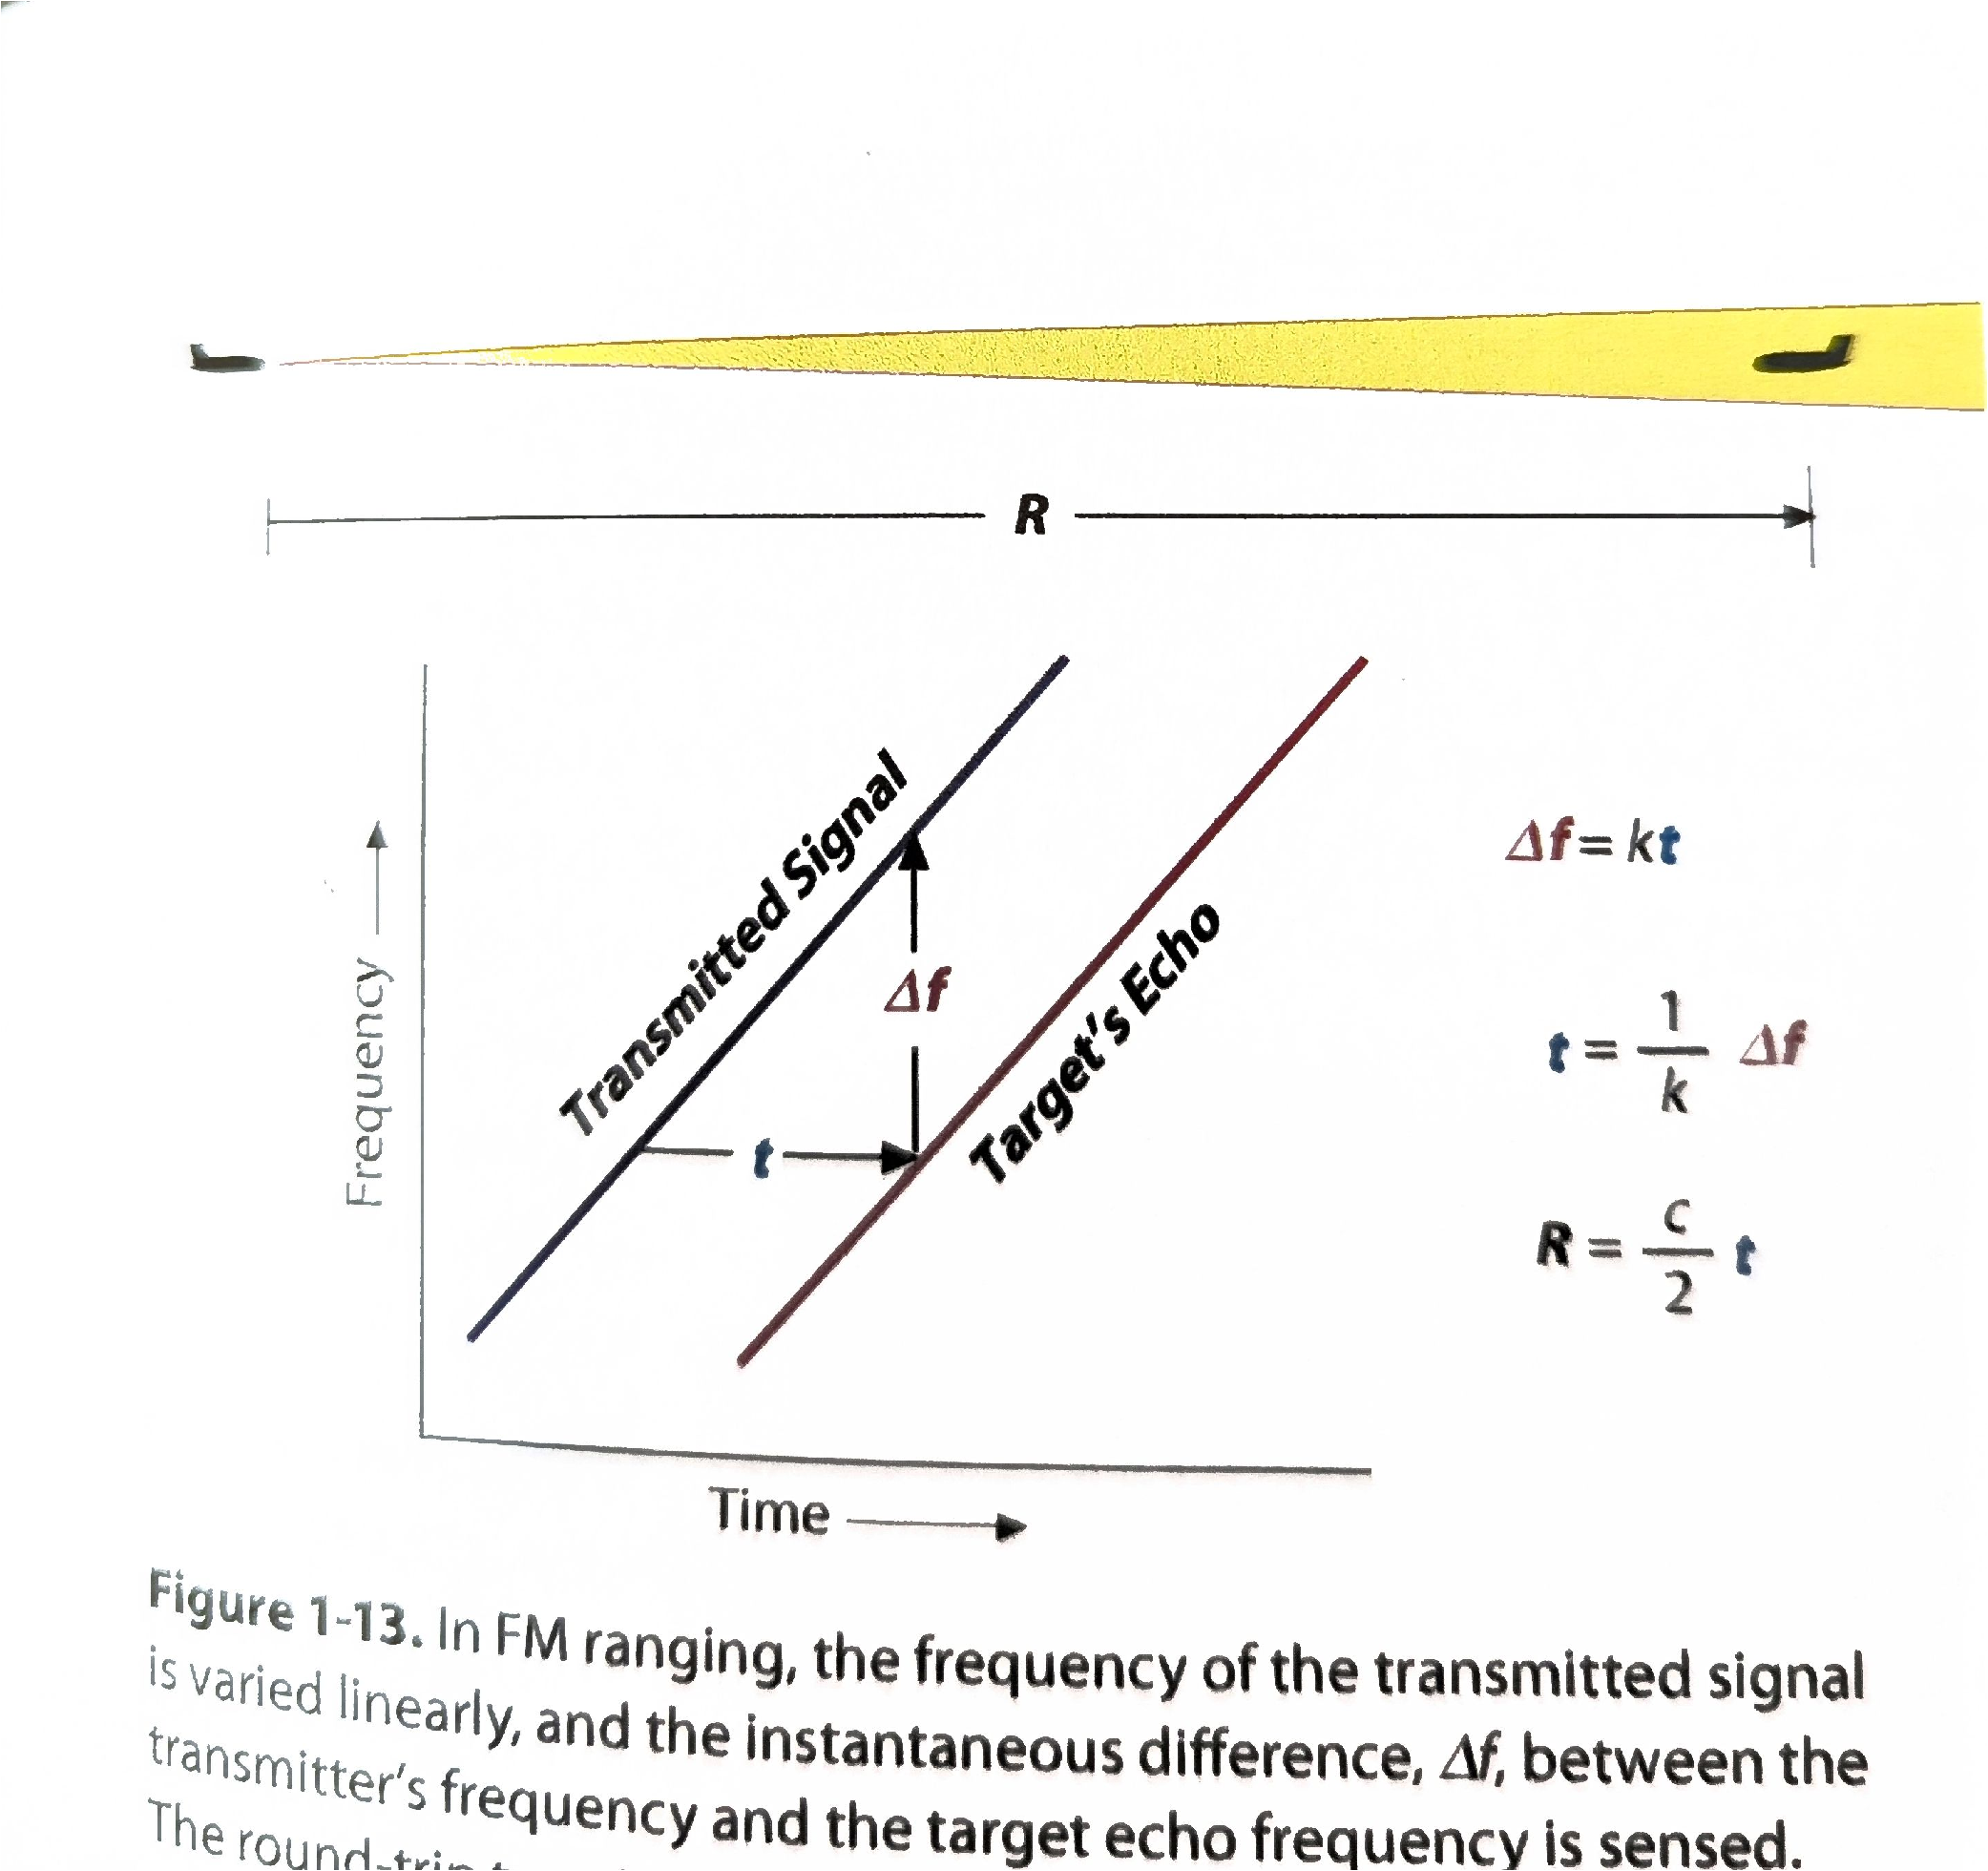
\includegraphics[width=0.5\textwidth,trim=2cm 6cm 2cm 3cm,clip=true]{radar.pdf}
\caption{\label{fig:1} In a basic chirping RF signal scheme used to detect enemy aircraft, a transmitted RF signal is linearly chirped.  Information in the radar echo can be used to find the range, $R$.}
\end{figure}

\section{Audio Processing}

\begin{enumerate}
\item \textbf{Bonus:} (a) Convert the data used to produce the radar spectrogram into audio data. (b) Filter the noise as appropriate, using the filter scheme of your choice. (c) Play the audio and listen for the two chirps.  Do the interfere and create a beat frequency?  Sometimes, $f_d$ in Doppler schemes is called the \textit{beat frequency.}
\end{enumerate}

\end{document}
